\documentclass[11pt, tikz]{standalone}
\usepackage{amsmath}
\usetikzlibrary{arrows.meta, decorations.pathmorphing, positioning, calc}
\usepackage{xcolor}

\definecolor{OliveGreen}{rgb}{0.33, 0.5, 0.18}
\definecolor{Blue}{rgb}{0.06, 0.2, 0.65}
\definecolor{keyword}{HTML}{8e4e9e}
\definecolor{myblue}{HTML}{3471d8}
\definecolor{type}{HTML}{4EC9B0}

\begin{document}
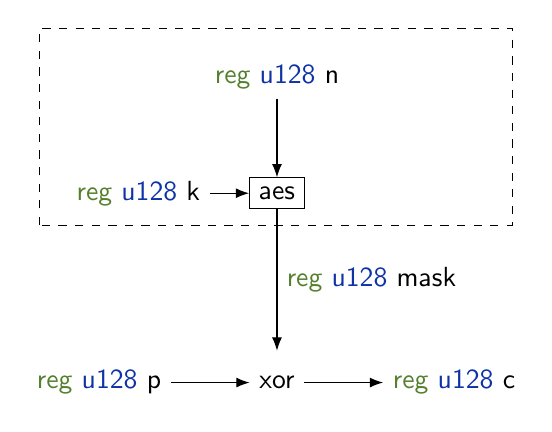
\begin{tikzpicture}[scale=1]\sffamily
	\tikzstyle{XOR} = [
	line width=.25mm,
	draw,
	circle,
	outer sep=2pt,
	append after command={
		[shorten >=2bp, shorten <=2bp]
		(\tikzlastnode.north) edge[line width=.25mm] (\tikzlastnode.south)
		(\tikzlastnode.east) edge[line width=.25mm] (\tikzlastnode.west)}
	]
	
	\node[] (pt) {\textcolor{OliveGreen}{reg} \textcolor{Blue}{u128} p};  
	\node[right=1cm of pt] (xor) {xor};
	\node[draw, rectangle, above=2cm of xor, align=center] (prf) {aes};
	\node[left=.5cm of prf] (key) {\textcolor{OliveGreen}{reg} \textcolor{Blue}{u128} k};
	\node[above=1cm of prf] (nonce) {\textcolor{OliveGreen}{reg} \textcolor{Blue}{u128} n};
	\node[right=1cm of xor] (ct) {\textcolor{OliveGreen}{reg} \textcolor{Blue}{u128} c};  
	\draw[dashed] (-.75,2) rectangle (5.25,4.5);
	
	\draw[-{Latex}] (pt) to (xor);
	\draw[-{Latex}] (xor) to (ct);
	\draw[-{Latex}] (prf) -- node[right] {\textcolor{OliveGreen}{reg} \textcolor{Blue}{u128} mask} ++ (0,-2);
	\draw[-{Latex}] (key) to (prf);
	\draw[-{Latex}] (nonce) to (prf);
	
	%	\node [below=of xor, align=left] {$\enc(k, n, m)=m\oplus f_k(n)$\\ $\dec(k, n, c)=c\oplus f_k(n)$};
\end{tikzpicture}
\end{document}
